\documentclass[]{standalone}

\usepackage{tikz}
\usetikzlibrary{
  calc,
  arrows, arrows.meta,
  positioning, intersections,
  patterns, patterns.meta,
}
\tikzset{
  dot/.style = {circle, fill=red!80!gray, minimum
      size=#1, draw=black,
      inner sep=0pt, outer sep=0pt},
  dot/.default = 5pt, % size of the circle diameter 
  wdot/.style = {dot=#1, fill=white},
  wdot/.default = 5pt, % size of the circle diameter 
  bdot/.style = {dot=#1, fill=black},
  bdot/.default = 5pt, % size of the circle diameter 
}

\begin{document}
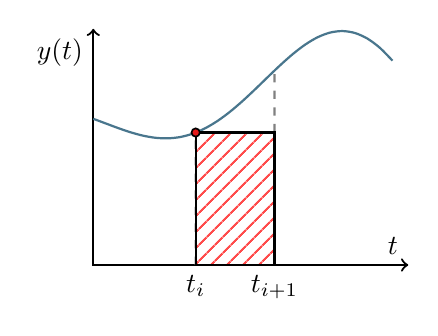
\begin{tikzpicture}[thick]
  \draw[to-to] (0,3) node[below left] {$y(t)$} |- (4,0) node[above left] {$t$};
  \draw[
    domain=0:3.8,
    smooth,
    variable=\x,
    cyan!50!black,
    name path=f1
  ] plot ({\x}, {2-(\x+.8)*sin(deg(\x*1.3+.8))/4});

  \coordinate (a) at (1.3, 0);
  \coordinate (b) at (2.3, 0);
  \coordinate (o) at (0,0);

  \node[below] at (a) {$t_{i}$};
  \node[below] at (b) {$t_{i+1}$};

  \draw[transparent, name path=f2] (a) -- ++(0,3);
  \path[name intersections={of=f1 and f2, by={at}}];
  \draw[transparent, name path=f3] (b) -- ++(0,3);
  \path[name intersections={of=f1 and f3, by={bt}}];


  \draw[dashed, gray] (a) -- (at);
  \draw[dashed, gray] (b) -- (bt);

  \filldraw[
    pattern = {Lines[angle=45,distance=4pt]},
    pattern color=red!70
  ] (at) rectangle (b);

  \node[dot = 3pt, semithick] at (at) {};
\end{tikzpicture}
\end{document}
